\section{Bestemmelse af vandtemperatur i rør}
Produktet skal kunne overvåge vandspildet uden at have regulerbare funktioner, dette efterlader muligheden af sammenligningen mellem overflade temperaturen på vandrøret og temperaturen i rummet, endvidere muligheden for at måle fugtigheden.  
\\
\\
\begin{figure}[h!]
  \centering
  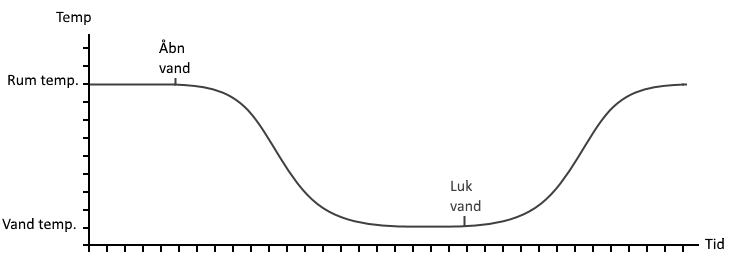
\includegraphics[width=0.7\textwidth]{figures/vandspild_graf_normal.png}
  \caption{Grafen viser overvågningssystemet uden vand spild.}
  \label{vandspild_graf_normal}
\end{figure}
\fxnote{ret figur, ingen grund til den er så høj når vi kun har 2 punkter på x aksen}
\\
\\
Figur \ref{vandspild_graf_normal} viser hvordan temperaturændringerne forekommer, hvis det antages at der ingen vandspild er og temperaturen på røret derfor er lig med temperaturen i rummet. I det der tilføres nyt vand til huset ændres rørets temperatur og der vil derfor forekomme temperatursvingninger for at kunne aflæse vandspildet.
\\
\\
\begin{figure}[h!]
  \centering
  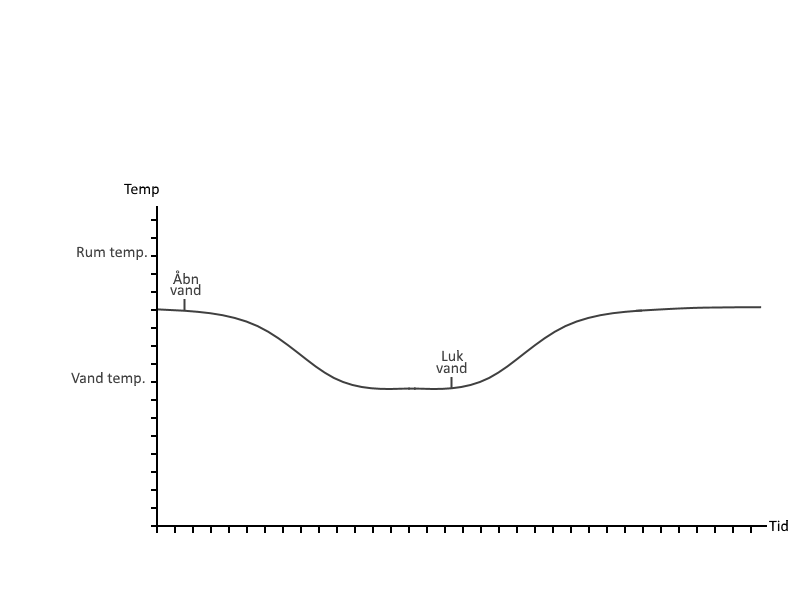
\includegraphics[width=0.7\textwidth]{figures/vandspild_graf_spild.png}
  \caption{Grafen viser overvågningssystemet med vandspild.}
  \label{vandspild_graf_spild}
\end{figure}
\fxnote{ret figur, ingen grund til den er så høj når vi kun har 2 punkter på x aksen}
\\
\\
Ovenstående figur \ref{vandspild_graf_spild} viser et eksempel på temperaturændringer ved vandspild på et rør. Her ses det hvordan hviletemperaturen på røret aldrig når temperaturen i rummet da vandet aldrig ligger helt stille og derfor tilfører en konstant koldere temperatur.  



    